%%
%% datosconceptual.tex
%% $Id: datosconceptual_acl2.tex 617 2008-06-28 17:00:10Z antonio $ 
%%

\subsubsection{Notaci�n}
\label{sec:conceptual_notacion}

Se ha usado \ac{UML} 2.0, con las siguientes modificaciones:
\begin{itemize}
\item Por claridad, algunas clases se hallan duplicadas en los
  diagramas. Para evitar confusiones, las duplicaciones ocultan los
  atributos y se hallan en color azul.
\item Igualmente, se han omitido las multiplicidades unitarias en las
  asociaciones y composiciones.
\end{itemize}

\subsubsection{Descripci�n general}
\label{sec:conceptual_acl2_general}

Para \postprocesador{}, los conceptos a tratar son entes abstractos
relacionados con el proceso de demostraci�n de \ac{ACL2}.

As�, partimos de un \clase{Enunciado}, colecci�n de \clase{Orden}es de
\ac{ACL2} que produce una \clase{Demostraci�n}. Esta
\clase{Demostraci�n} asocia a cada \clase{Orden} un \clase{Resultado}
con la salida obtenida de \ac{ACL2}. Esta contendr� diversos tipos de
informaci�n seg�n la \clase{Orden} usada.

Puede que nuestro \clase{Enunciado} sea la ra�z de un proyecto de
\ac{ACL2}, y se halle definido en base a una serie de definiciones ya
demostradas en \clase{Libro}s existentes. Es importante ver que un
\clase{Libro} puede requerir de una serie de definiciones previas a su
vez: seg�n la terminolog�a de \ac{ACL2}, ser�a su \emph{mundo
  inicial}. Todo \clase{Evento} pertenece a un \clase{Paquete}: si no
se indica su nombre previamente con una orden \orden{in-package}, ser�
``ACL2''.

Adicionalmente, pueden aparecer avisos, errores y observaciones de
\ac{ACL2} al inicio del resultado de la ejecuci�n de una \clase{Orden}
dada.

A su vez, cada \clase{Resultado}, en caso de necesitar demostrar
alguna S-expresi�n, usar� una \clase{Meta} principal, que se podr�
dividir recursivamente en submetas. Cada \clase{Meta} usa un
determinado \clase{Proceso} de demostraci�n.

Se ha dividido el diagrama de clases conceptuales en tres:
\begin{enumerate}
\item Visi�n general del dominio del problema:
  figura~\ref{fig:conceptual_general} de la
  p�gina~\pageref{fig:conceptual_general}.

\item Tipos de Orden: figura~\ref{fig:conceptual_ordenes} de la
  p�gina~\pageref{fig:conceptual_ordenes}.

  Es interesante ver c�mo algunas �rdenes utilizan a otras. Por
  ejemplo, como paso de verificaci�n tras la certificaci�n de un libro
  con \orden{certify-book}, se intentan cargar sus contenidos en el
  mundo de \ac{ACL2}, justo como si se hubiera ejecutado una orden
  \orden{include-book}.

\item Tipos de Proceso: figura~\ref{fig:conceptual_procesos} de la
  p�gina~\pageref{fig:conceptual_procesos}.

\end{enumerate}

\begin{sidewaysfigure}
  \centering
  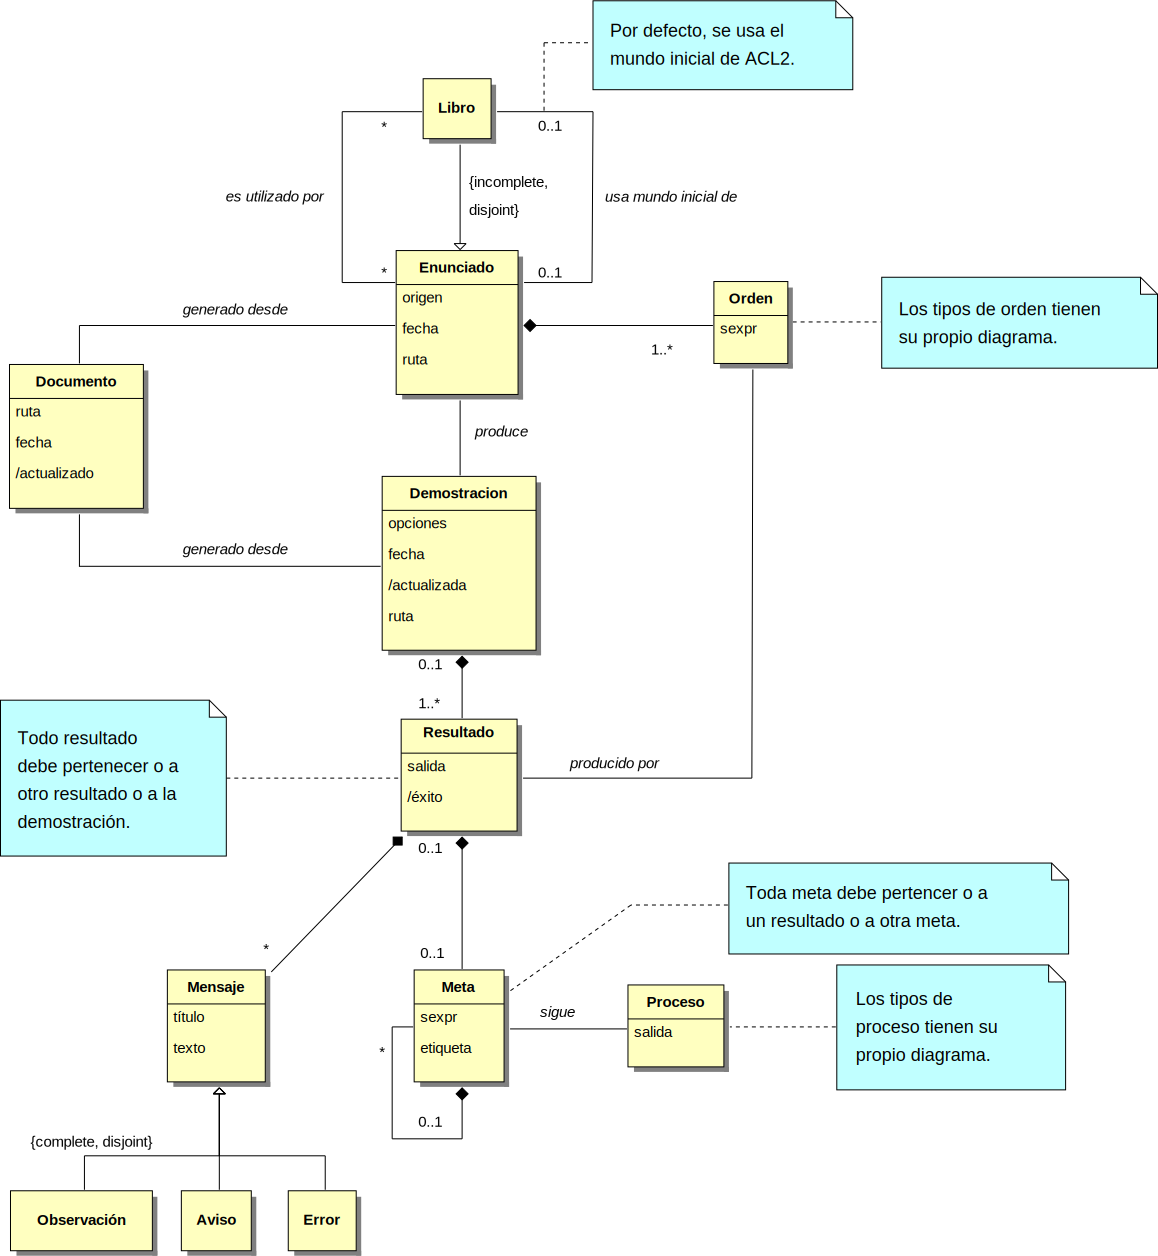
\includegraphics[height=.7\textheight]{desarrollo/analisis/modacl2_general}
  \caption{Diagrama de clases conceptuales general de \acs{ACL2}}
  \label{fig:conceptual_general}
\end{sidewaysfigure}

\begin{sidewaysfigure}
  \centering
  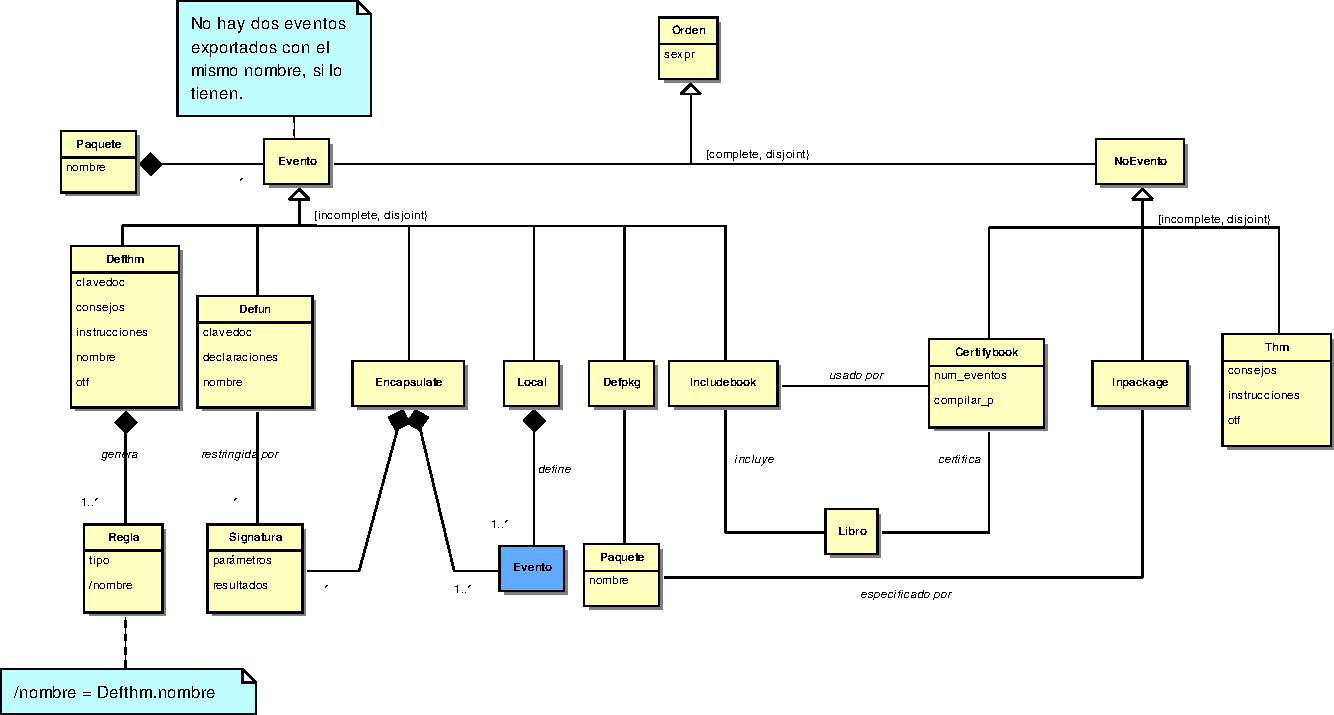
\includegraphics[width=\textwidth]{desarrollo/analisis/modacl2_ordenes}
  \caption{Diagrama de clases conceptuales de �rdenes de \acs{ACL2}}
  \label{fig:conceptual_ordenes}
\end{sidewaysfigure}

\begin{sidewaysfigure}
  \centering
  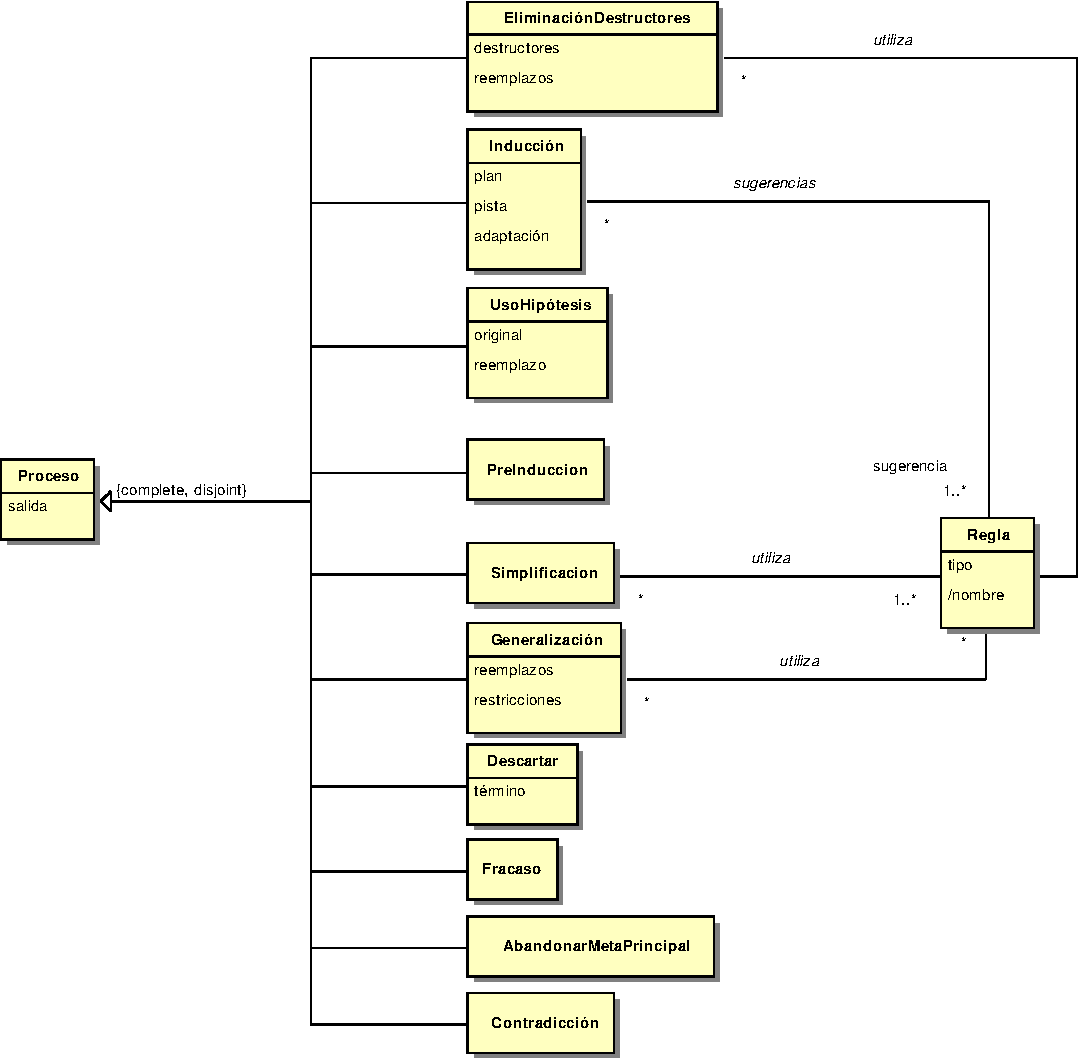
\includegraphics[height=.7\textheight]{desarrollo/analisis/modacl2_procesos}
  \caption{Diagrama de clases conceptuales de procesos de \acs{ACL2}}
  \label{fig:conceptual_procesos}
\end{sidewaysfigure}

\subsubsection{Restricciones textuales}

\begin{enumerate}
\item \emph{Clave externa}: ``nombre'' de \clase{Documento}.
\item \emph{Clave externa}: ``nombre'' de \clase{Paquete}.
\item \emph{Clave externa}: ``nombre'' de cualquier descendiente de
  \clase{Evento}, si lo tiene.
\item \emph{Clave externa}: ``clavedoc'' de cualquier descendiente de
  \clase{Evento}, si la tiene y est� especificada.
\item Todo \clase{Resultado} pertenece o a otro \clase{Resultado} o a una
  \clase{Demostraci�n}.
\item Todo \clase{Meta} pertenece o a otra \clase{Meta} o a un \clase{Resultado}.
\item Toda \clase{Meta} tiene una etiqueta �nica dentro de una \clase{Demostraci�n}.
\item \clase{Resultado}.�xito $\in{} \left\{ \text{verdadero},
    \text{falso} \right\}$.
\item \clase{Documento}.actualizado $\in{} \left\{ \text{verdadero},
    \text{falso} \right\}$.
\item \clase{Demostraci�n}.actualizada $\in{} \left\{ \text{verdadero},
    \text{falso} \right\}$.
\end{enumerate}

\subsubsection{Derivaciones}

\begin{enumerate}
\item \clase{Demostraci�n}.actualizada = ``verdadero'' si
  \clase{Demostraci�n}.fecha es una fecha y hora posterior a
  \clase{Enunciado}.fecha. ``falso'' de lo contrario.
\item \clase{Documento}.actualizado = ``verdadero'' si
  \clase{Demostraci�n}.actualizada y \clase{Documento}.fecha es una
  fecha y hora posterior a \clase{Demostraci�n}.fecha. ``falso'' de lo
  contrario.
\item \clase{Resultado}.�xito = no contiene \clase{Meta} con el
  \clase{Proceso} \clase{Fracaso} y sus \clase{Resultados} de inferior
  nivel (si los hay) tienen �xito.
\item \clase{Regla}.nombre = \clase{Defthm}.nombre.
\end{enumerate}

%%% Local Variables: 
%%% mode: latex
%%% TeX-master: "../../memoria"
%%% End: 
